\documentclass[a4paper]{article}
%
\usepackage[utf8]{inputenc}
\usepackage[T1]{fontenc}
\usepackage[english]{babel}
\usepackage{amsmath,esint}
\usepackage{amssymb,amsfonts,textcomp}
\usepackage{color}
\usepackage[top=2.54cm,bottom=1.251cm,left=2.54cm,right=2.54cm,nohead,includefoot,foot=1.289cm,footskip=2.4780002cm]{geometry}
\usepackage{array}
\usepackage{supertabular}
\usepackage{hhline}
\usepackage{hyperref}
\hypersetup{colorlinks=true, linkcolor=blue, citecolor=blue, filecolor=blue, urlcolor=blue, pdftitle=Implementation of the electromagnetic diffusion model of canonical test cases using the finite element method, pdfauthor=Ian Flintoft, pdfkeywords=power balance; diffusion; statistical energy balance}
\usepackage[pdftex]{graphicx}
\usepackage[nottoc]{tocbibind}
\usepackage{stmaryrd}
\usepackage{natbib}
\setcitestyle{authoryear,open={(},close={)}}
%\usepackage{times}
%\usepackage{fancyhdr}
\usepackage[reqno]{empheq}
%\usepackage{txfonts}
\usepackage{doi}
%
%====================================================================
%-------------------------------------------------------------------- 
%
%   isomath.tex  LaTeX macros for math conforming to ISO standards
%
%---------------------------------------- this is a LaTeX-2e document
%====================================================================     

%% Blackboard Bold

\newcommand*{\bbb}[1]{\mathbb{#1}}
\newcommand{\bC}{\bbb{C}}
\newcommand{\bN}{\bbb{N}}
\newcommand{\bQ}{\bbb{Q}}
\newcommand{\bR}{\bbb{R}}
\newcommand{\bZ}{\bbb{Z}}
\newcommand{\bF}{\bbb{F}}
\newcommand{\bFp}{\bbb{F}_p}
\newcommand{\bFpn}{\bbb{F}_{p^n}}
\newcommand{\ii}{\mathbf{i}}
\newcommand{\jj}{\mathbf{j}}
\newcommand{\kk}{\mathbf{k}}

\newcommand{\N}{\bN}
\newcommand{\Q}{\bQ}
\newcommand{\R}{\bR}
\newcommand{\Z}{\bZ}
\newcommand{\ZpZ}{\Z/p\Z}
\newcommand{\ZmZ}{\Z/m\Z}
\newcommand{\C}{\bC}
\newcommand{\F}{\bF}
\newcommand{\Fp}{\bFp}
\newcommand{\Fpn}{\bFpn}

%% Calligraphic

\renewcommand*{\cal}[1]{\mathcal{#1}}
\newcommand{\cQ}{\cal{Q}}
%\newcommand{\cC}{\cal{C}}
%\newcommand{\cF}{\cal{F}}
%\newcommand{\cH}{\cal{H}}
%\newcommand{\cK}{\cal{K}}
%\newcommand{\cT}{\cal{T}}

%% Named Functions and Operators
\newcommand{\id}{\mathrm{id}}
\newcommand{\Id}{\mathrm{Id}}
\newcommand{\rank}{\mathrm{rank}}
\newcommand{\tr}{\mathrm{tr}}
\newcommand{\Aut}{\mathrm{Aut}}
\renewcommand{\Re}{\ensuremath{\mathrm{Re}}}
\renewcommand{\Im}{\ensuremath{\mathrm{Im}}}

\DeclareMathOperator{\cod}{Codom}
\DeclareMathOperator{\dom}{Dom}
\DeclareMathOperator{\im}{Im}
\DeclareMathOperator{\ran}{Ran}
\DeclareMathOperator{\supp}{supp}

\DeclareMathOperator*{\clsp}{\overline{span}}
\DeclareMathOperator*{\spn}{span}

%% Vectors

\usepackage{amsbsy}
\renewcommand*{\vec}[1]{\boldsymbol{\mathrm{#1}}}
\newcommand{\va}{\vec{a}}
\newcommand{\vb}{\vec{b}}
\newcommand{\vc}{\vec{c}}
\newcommand{\ve}{\vec{e}}
\newcommand{\vf}{\vec{f}}
\newcommand{\vk}{\vec{k}}
\newcommand{\vl}{\vec{l}}
\newcommand{\vm}{\vec{m}}
\newcommand{\vn}{\vec{n}}
\newcommand{\vp}{\vec{p}}
\newcommand{\vr}{\vec{r}}
\newcommand{\vs}{\vec{s}}
\newcommand{\vx}{\vec{x}}
\newcommand{\vy}{\vec{y}}
\newcommand{\vz}{\vec{z}}
\newcommand{\vu}{\vec{u}}
\newcommand{\vv}{\vec{v}}
\newcommand{\vw}{\vec{w}}
\newcommand{\vA}{\vec{A}}
\newcommand{\vE}{\vec{E}}
\newcommand{\vG}{\vec{G}}
\newcommand{\vH}{\vec{H}}
\newcommand{\vI}{\vec{I}}
\newcommand{\vD}{\vec{D}}
\newcommand{\vB}{\vec{B}}
\newcommand{\vF}{\vec{F}}
\newcommand{\vJ}{\vec{J}}
\newcommand{\vM}{\vec{M}}
\newcommand{\vP}{\vec{P}}
\newcommand{\vQ}{\vec{Q}}
\newcommand{\vS}{\vec{S}}
\newcommand{\vtimes}{\vec{\times}}
\newcommand{\vcdot}{\vec{\cdot}}
\newcommand{\vnabla}{\vec{\nabla}}
\newcommand{\valpha}{\vec{\alpha}}
\newcommand{\vtheta}{\vec{\theta}}
\newcommand{\vphi}{\vec{\phi}}
\newcommand{\vzero}{\vec{0}}
\newcommand{\vrho}{\vec{\rho}}
\newcommand{\vvarepsilon}{\vec{\varepsilon}}

%% Normalised fields

\newcommand{\tE}{\tilde{E}}
\newcommand{\tH}{\tilde{H}}
\newcommand{\tP}{\tilde{E}}
\newcommand{\tPP}{\tilde{P'}}
\newcommand{\tB}{\tilde{B}}
\newcommand{\tM}{\tilde{M}}
\newcommand{\tJ}{\tilde{J}}
\newcommand{\tDelta}{\tilde{\Delta}}
\newcommand{\tbeta}{\tilde{\beta}}
\newcommand{\tgamma}{\tilde{\gamma}}
\newcommand{\talpha}{\tilde{\alpha}}
\newcommand{\bbeta}{\bar{\beta}}
\newcommand{\bgamma}{\bar{\gamma}}
\newcommand{\balpha}{\bar{\alpha}}

%% Logical Propositions

\newcommand*{\pro}[1]{\mathsf{#1}}
\newcommand{\pP}{\pro{P}}
\newcommand{\pQ}{\pro{Q}}
\newcommand{\pR}{\pro{R}}

%% Matrices and Tensors

\DeclareMathAlphabet{\mathsfsl}{OT1}{cmss}{m}{sl}
\newcommand*{\mat}[1]{\mathsfsl{#1}}
\newcommand{\mA}{\mat{A}}
\newcommand{\mD}{\mat{D}}
\newcommand{\mH}{\mat{H}}
\newcommand{\mI}{\mat{I}}
\newcommand{\mM}{\mat{M}}
\newcommand{\mO}{\mat{O}}
\newcommand{\mP}{\mat{P}}
\newcommand{\mQ}{\mat{Q}}
\newcommand{\mR}{\mat{R}}
\newcommand{\mS}{\mat{S}}
\newcommand{\mT}{\mat{T}}
\newcommand{\mU}{\mat{U}}
\newcommand{\mY}{\mat{Y}}
\newcommand{\mZ}{\mat{Z}}

%% Special Numbers and Characters

\newcommand{\ra}{\mathrm{a}}
\newcommand{\rc}{\mathrm{c}}
\newcommand{\re}{\mathrm{e}}
\newcommand{\rf}{\mathrm{f}}
\newcommand{\rh}{\mathrm{h}}
\newcommand{\ri}{\mathrm{i}}
\newcommand{\rrm}{\mathrm{m}}
\newcommand{\ro}{\mathrm{o}}
\newcommand{\rp}{\mathrm{p}}
\newcommand{\rr}{\mathrm{r}}
\newcommand{\rs}{\mathrm{s}}
\newcommand{\rd}{\mathrm{d}} % differential
\newcommand{\rt}{\mathrm{t}}
\newcommand{\rw}{\mathrm{w}}
\newcommand{\rz}{\mathrm{z}}
\newcommand{\rA}{\mathsf{A}}
\newcommand{\rE}{\mathsf{E}}
\newcommand{\rF}{\mathsf{F}}
\newcommand{\rG}{\mathrm{G}}
\newcommand{\rH}{\mathrm{H}}
\newcommand{\rI}{\mathrm{I}}
\newcommand{\rK}{\mathrm{K}}
\newcommand{\rL}{\mathrm{L}}
\newcommand{\rM}{\mathrm{M}}
\newcommand{\rN}{\mathrm{N}}
\newcommand{\rO}{\mathrm{O}}
\newcommand{\rP}{\mathrm{P}}
\newcommand{\rR}{\mathrm{R}}
\newcommand{\rS}{\mathrm{S}}
\newcommand{\rT}{\mathrm{T}}
\newcommand{\rU}{\mathrm{U}}
\newcommand{\rV}{\mathrm{V}}
\newcommand{\rW}{\mathrm{W}}
\newcommand{\rX}{\mathrm{X}}
\newcommand{\rY}{\mathrm{Y}}
\newcommand{\rZ}{\mathrm{Z}}

%\newcommand{\rpi}{\pi}       % actually, pi should be upright.
\newcommand{\rpi}{\piup}      % like this - needs txfonts package!

\newcommand{\dif}[1]{\,\rd{#1}} % differential
\newcommand{\df}{\dif{f}}
\newcommand{\dx}{\dif{x}}
\newcommand{\dy}{\dif{y}}
\newcommand{\dz}{\dif{z}}
\newcommand{\dt}{\dif{t}}
\newcommand{\deriv}[3][]{\frac{\rd^{#1}#2}{\rd #3^{#1}}}           % total derivative
\newcommand{\pderiv}[3][]{\frac{\partial^{#1}#2}{\partial #3^{#1}}} % partial derivative

\renewcommand{\jmath}{\mathrm{j}\mkern1mu}

%% Units
\newcommand*{\unit}[1]{\ensuremath{\mathrm{\,#1}}}
\newcommand{\degree}{\ensuremath{^\circ}}
\newcommand{\celsius}{\ensuremath{^\circ C}}
\newcommand{\micro}{\ensuremath{\mu}}
\newcommand{\ohm}{\ensuremath{\mathrm{\Omega}}}

%% Shortcuts
\newcommand{\prt}{(\vr,t)}
\newcommand{\pr}{(\vr)}
\newcommand{\prw}{(\vr,\omega)}
\newcommand{\epsilonc}{\hat{\epsilon}}

%% Unit vectors
\newcommand{\uve}{\widehat{\ve}}
\newcommand{\uvx}{\widehat{\vx}}
\newcommand{\uvy}{\widehat{\vy}}
\newcommand{\uvz}{\widehat{\vz}}
\newcommand{\uvk}{\widehat{\vk}}
\newcommand{\uvn}{\widehat{\vn}}
\newcommand{\uvp}{\widehat{\vp}}
\newcommand{\uvr}{\widehat{\vr}}
\newcommand{\uvtheta}{\widehat{\vtheta}}
\newcommand{\uvepsilon}{\widehat{\vvarepsilon}}
\newcommand{\uvphi}{\widehat{\vphi}}
\newcommand{\uvrho}{\widehat{\vrho}}

%====================================================================

\numberwithin{equation}{section}
\makeatletter
\newcommand\arraybslash{\let\\\@arraycr}
\makeatother
% Footnote rule
\setlength{\skip\footins}{0.119cm}
\renewcommand\footnoterule{\vspace*{-0.018cm}\setlength\leftskip{0pt}\setlength\rightskip{0pt plus 1fil}\noindent\textcolor{black}{\rule{0.25\columnwidth}{0.018cm}}\vspace*{0.101cm}}
\setlength\tabcolsep{1mm}
\renewcommand\arraystretch{1.3}
\newcounter{Table}
\renewcommand\theTable{\arabic{Table}}
\newcounter{Figure}
\renewcommand\theFigure{\arabic{Figure}}
\providecommand\oiint{\oint}
\newcommand*{\defeq}{\stackrel{\text{def}}{=}}
%
\title{Implementation of the electromagnetic diffusion model of canonical test cases using the finite element method}
\author{Ian Flintoft}
\date{2017-02-04}
%
\begin{document}
\clearpage\setcounter{page}{1}{\centering
\textbf{\Large Implementation of the electromagnetic diffusion model of canonical test cases using the finite element method}
\par}
\vspace{5mm}
{\centering\large 
Ian Flintoft\footnote{ Email: \href{mailto:ian.flintoft@googlemail.com}{ian.flintoft@googlemail.com}; 
Web: \url{https://idflintoft.bitbucket.io}}, University of York
\par}
\vspace{5mm}
{\centering
04 February 2017
\par}
\vspace{5mm}
\textbf{\textit{Abstract}}\textit{ -- These notes provide details of the implementation of the 
electromagnetic diffusion model of some canonical test cases using the finite element method.
The treatment is terse and no attempt has been made to motivate the methods used or to provide
comprehensive background and references. 
}
%
\setcounter{tocdepth}{3}
\renewcommand\contentsname{Contents}
\tableofcontents
%

\section[Glossary and symbols]{Glossary and symbols}
\label{sc:gloss}

%\begin{center}
\begin{supertabular}{m{2cm}l}
%\hline
%\textbf{Acronym} &\textbf{Definition} \\
%\hline
ACS              & (Average) Absorption Cross-Section  \\
AE               &(Average) Absorption Efficiency      \\
EC               &(Energy) Exchange Coefficient        \\
EM               &Electromagnetic                      \\
FE               &Finite Element                       \\
FEM              &Finite Element Method                \\
MFP              &Mean-Free-Path                       \\
ODE              &Ordinary Differential Equation       \\
PDE              &Partial Differential Equation        \\
PWB              &Power Balance                        \\
TCS              &(Average) Transmission Cross-Section \\
TE               &(Average) Transmission Efficiency    \\
%\hline
\end{supertabular}
%\end{center}
\vspace{5mm}

\begin{center}
\begin{supertabular}{|c|c|c|l|}
\hline
\textbf{Symbol}     &\textbf{Unit}   &\textbf{Variable}    &\textbf{Definition} \\
\hline
$w\prt$             &J\,m$^{-3}$     &\texttt{w}           &Spatial and temporal average energy density in cavity \\
$D\pr$              &m$^2$\,s$^{-1}$ &\texttt{D}           &Diffusivity \\
$\Lambda _V$        &s$^{-1}$        &-                    &Volumetric absorption loss rate \\
$p\prt$             &W\,m$^{-3}$     &~                    &Volumetric power density source \\
$\rc_0$             &m\,s${-1}$      &\texttt{c0}          &Speed of light in free-space \\
$\lambda$           &m               &\texttt{MFP}         &Mean free path \\
$\vJ\prt$           &W\,m$^{-2}$     &\texttt{J}           &Fickian energy density flux \\
$V$                 &m$^3$           &\texttt{V}           &Domain volume \\
$S$                 &m$^2$           &\texttt{S}           &Domain surface area \\
$\kappa$            &-               &\texttt{specularity} &Empirical specular correction factor for diffusivity \\
$h\pr$              &m\,s$^{-1}$     &\texttt{EC}          &Energy exchange coefficient of domain boundary \\
$\alpha\pr$         &-               &\texttt{AE}          &Average absorption efficiency of domain boundary \\
$\uvn$              &-               &-                    &Outward unit normal vector for domain \\
$\lambda_\rw$       &m               &\texttt{wallMFP}     &Mean free path for wall scattering \\
$D_\rw$             &m$^2$\,s$^{-1}$ &\texttt{wallD}       &Diffusivity for wall scattering \\
$\alpha_\rw\pr$     &~               &\texttt{wallAE}      &Average absorption efficiency of walls \\
$h_\rw\pr$          &m\,s$^{-1}$     &\texttt{wallEC}      &Energy exchange coefficient of walls \\
$\lambda _\rf$      &m               &\texttt{fittingMFP}  &Mean free path for fitting scattering \\
$D_\rf$             &m$^2$\,s$^{-1}$ &\texttt{fittingD}    &Diffusivity path for fitting scattering \\
$\alpha_\rf\pr$     &-               &\texttt{fittingAE}   &Average absorption efficiency of fittings \\
$\sigma_\rf^\rs$    &m$^2$           &\texttt{fittingSCS}  &Average scattering cross-section of fittings \\
$h_\rf\pr$          &m\,s$^{-1}$     &\texttt{fittingEC}   &Energy exchange coefficient of fittings \\
$n_V^\rf$           &m$^{-3}$        &~                    &Volumetric number density of fittings \\
$\Lambda_V^\rf$     &s$^{-1}$        &~                    &Volumetric absorption loss rate due to fittings \\
$P^\rt$             &W               &\texttt{TRP}         &Source total (isotropic) radiated power \\
$V_\rs$             &m$^3$           &\texttt{srcVolume}   &Volume source volume \\
$S_\rs$             &m$^2$           &\texttt{srcArea}     &Surface source surface area \\
$J_\rs$             &W\,m$^{-2}$     &\texttt{srcExitance} &Surface source exitance \\
$\tau$              &-               &\texttt{TE}          &Average transmission efficiency of lossless aperture \\
$w_\rr\prt$         &J\,m$^{-3}$     &\texttt{wr}          &Average reverberant energy density in cavity \\
$J_\rr\prt$         &W\,m$^{-2}$     &\texttt{Jr}          &Reverberant energy density flux \\
$S\prt$             &W\,m$^{-2}$     &\texttt{S}           &Average scalar power density \\
\hline
\end{supertabular}
\end{center}

\section[Summary of the model]{Summary of the model}
\label{sc:sum}

\subsection[The diffusion equation]{The diffusion equation}
\label{sc:sum:edm}

In the electromagnetic diffusion model (EDM) the diffuse electromagnetic energy
density, $w\prt$, at position $\vr$ and time $t$ in a closed
domain $\Omega$ is assumed to satisfy the diffusion equation
\begin{align}
\begin{matrix}
\frac{\partial w\prt}{\partial t} - \vnabla\vcdot\left[D\pr \vnabla w\prt \right] + \Lambda_V w\prt = p\prt &\vr\in\Omega 
\end{matrix}
\end{align}
where $D\prt$ is the potentially inhomogeneous diffusivity, $\Lambda_V$ is an 
overall volumetric absorption loss rate and  $p\prt$ is the volume power density 
of any sources. This is a second order parabolic partial differential equation (PDE).
For time dependent problems the initial value of the energy density must be
prescribed over the volume
\begin{align}
\begin{matrix}
\left.w\prt\right|_{t_0} = w_0\pr &\vr\in\Omega
\end{matrix}
\end{align}
The diffusivity accounts for the scattering within the cavity. To first
approximation it may be regarded as constant and is related to the
mean-free-path (MFP) between scattering events, $\lambda$, by
\begin{align}
D = \frac{1}{3}\rc_0\lambda 
\end{align}
where $\rc_0$ is the speed of light in free-space. 

The transport of average energy density is described by Fick’s law for the
energy density flux
\begin{align}
\vJ\prt = -D\pr\vnabla w\prt .
\end{align}
The diffusion equation can therefore be interpreted as an equation of continuity
\begin{align}
\begin{matrix}
\frac{\partial w\prt}{\partial t} +\vJ\prt + \Lambda_V w\prt= p\prt &\vr{\in}\Omega
\end{matrix}
\end{align}

\subsection[Scattering from the cavity walls]{Scattering from the cavity walls}
\label{sc:sum:walls}

For an empty cavity without a strong aspect ratio (i.e. one that is approximately cubic) 
the MFP for scattering from the walls is given by
\begin{align}
\lambda_\rw = \frac{4V}{S},
\end{align}
where $V$ and $S$ are the interior volume and surface area of the cavity
walls:
\begin{align}
V &= \iiint_{\Omega }\dif{V} \\
S &= \oiint_{\partial\Omega }\dif{S} .
\end{align}
For cavities with one dimension much greater than the others a better estimate
of the mean-free-path is given by
\begin{align}
\lambda_\rw = \sqrt{\frac{S}{4\pi}} .
\end{align}

{\color{red}Question: Is there any guidance as to when the aspect ratio is large enough that
this model is better?}

\subsection[Scattering and absorption from fittings]{Scattering and absorption from fittings}
\label{sc:sum:fit}

If there are objects (fittings) in the cavity the overall MFP is the harmonic
mean of the MFP of the walls and fittings,
\begin{align}
\frac{1}{\lambda} = \frac{1}{\lambda_\rw} + \frac{1}{\lambda_\rf},
\end{align}
as is the corresponding diffusivity
\begin{align}
\frac{1}{D} = \frac{1}{D_\rw} + \frac{1}{D_\rf},
\end{align}
The diffusivity is therefore dominated by the shortest MFP. The MFP for
scattering with identical of fittings of surface area $S_\rf$ and volumetric
concentration $n_V^\rf=N_\rf/V$ can be estimated as
\begin{align}
\lambda_\rf = \frac{1}{\sigma_\rf^\rs n_V^\rf} = \frac{4V}{S_\rf N_\rf},
\end{align}
where $\sigma_\rf^s=S_\rf/4$ is the average scattering cross-section of the
fittings. If the fittings are lossy then a term
\begin{align}
\Lambda_V^\rf = \frac{\rc_0\alpha_\rf}{\lambda_\rf}
\end{align}
must also be added to the volumetric scattering rate $\Lambda_V$ that accounts
for volumetric absorption processes. Here $\alpha_\rf$ is the average
absorption efficiency of the fittings.

Attempts have also been made to include the effects of specular reflections by
introducing an empirical factor, ${\kappa}$, into the diffusivity 
\begin{align}
D \rightarrow \kappa D
\end{align}
with $1\leq\kappa\lesssim 5$. 

{\color{red} Question: How strong is evidence for this and what is guidance on choosing the
value?}

{\color{red} Question: How do we determine the diffusivity in cases with complex topology such as
the test case with the cylinder? Empirically it appears the diffusivity is about one quarter of that
of the empty sub-cavity in the dutal cavity case. In the single cavity case the effect is not
noticable. The fitting method of determining MFP_fitting = 4S/S_fitting does not appear to be
appropriate for single contents which significiantly perturb the cavity shape.}

\subsection[Absorption in the cavity walls]{Absorption in the cavity walls}
\label{sc:sum:abs}

Absorption in the domain boundary are described by inhomogeneous Robin (also
called Fourier or Type 3) boundary conditions:
\begin{align}
\begin{matrix}
\uvn\vcdot\left[D\pr\vnabla w\prt\right] + h\pr w\prt = 0 &\vr\in\partial\Omega
\end{matrix}
\end{align}
where $\uvn$ is an outward normal vector to the domain and 
$h\pr$ is an energy exchange coefficient (EC). Various models have been
used in the acoustics literature to related the exchange coefficient to the
average absorption efficiency of the domain boundary, $\alpha\pr$. The
simplest uses the Sabine estimate of reverberation time giving
\begin{align}
\begin{matrix}
h\pr = \frac{1}{4}\rc_0\alpha \left(r\right)&0\leq\alpha\lesssim 0.2
\end{matrix}
\end{align}
and is regarded in acoustics as accurate only for low absorption $\alpha\lesssim 0.2$. 
A modified form based on the Eyring reverberation time has also been applied giving
\begin{align}
\begin{matrix}
h\pr = -\rc_0\frac{\log_{10}\left(1-\alpha\pr\right)}{4} &0\leq\alpha\lesssim 0.5
\end{matrix},
\end{align}
which empirically provides better results for moderate absorption, $\alpha\lesssim 0.5$, 
but becomes singular for $\alpha=1$. More recently a relation based on
a radiative transport model has been proposed which appears to give good
results over the full range of absorption
\begin{align}
\begin{matrix}
h\pr =\rc_0\frac{\alpha\pr}{2\left(2-\alpha\pr\right)} & 0\leq\alpha\leq 1 .
\end{matrix}
\end{align}

The absorption efficiencies and exchange coefficients for the walls and fittings
are denoted by $\alpha_\rw\pr$ and $\alpha_\rf\pr$ and 
$h_\rw\pr$ and $h_\rf\pr$ respectively.

\subsection[Sources]{Sources}
\label{sc:sum:src}

A point source of instantaneous total radiated power (TRP) $P^\rt(t)$
located at $\vr_\rs$ can be implemented as
\begin{align}
p\prt = P^\rt(t) \delta^{(3)}\left(\vr-\vr_\rs\right).
\end{align}
The energy density near such a source contains a spurious direct term that can
be subtract to give the reverberant energy density
\begin{align}
w_\rr\pr = w\pr - \frac{P^\rt}{4\pi D\left|\vr-\vr_\rs\right|}.
\end{align}
The true direct energy density is
\begin{align}
w_\rd\pr = \frac{P^\rt}{4\pi\rc_0\left|\vr-\vr_\rs\right|^2}.
\end{align}
The reverberant energy density flux is
\begin{align}
\vJ_\rr\prt = -D\vnabla w_\rr\pr = \vJ\prt - \frac{P^\rt}{4\pi\left|\vr-\vr_\rs\right|^3}\left(\vr-\vr_\rs\right).
\end{align}

A uniform volumetric source over a sub-domain $\Omega _s$ can be implemented
using
\begin{align}
\begin{matrix} 
p\prt = \frac{P^\rt(t)}{V_s} &\vr\in\Omega_\rs 
\end{matrix} \\
V_s = \iiint_{\Omega_\rs}\dif{V}
\end{align}
The spurious direct energy density from such source is less than for point
sources.

A portion of the domain boundary $\partial\Omega_\rs$ can also be used as a
surface source
\begin{align}
\begin{matrix}
\uvn\vcdot\left[D\pr\vnabla w\prt\right] - J_\rs\prt = 0 &\vr\in\partial\Omega_\rs
\end{matrix}
\end{align}
where
\begin{align}
J_\rs\prt &= \frac{P^\rt(t)}{S_\rs} \\
S_\rs &= \oiint_{\partial\Omega_\rs}\dif{S} .
\end{align}

\subsection[Coupled domains]{Coupled domains}
\label{sc:sum:coup}

Consider the case of two cavities of domains $\Omega_1$ and $\Omega_2$ with
diffusivities $D_1\pr$ and $D_2\pr$ coupled by a translucent part of their 
shared boundary; the domain 1 side of the shared boundary is denoted by 
${\partial}\Omega_{12}$ and the domain 2 side by ${\partial}\Omega_{21}$.
If the coupling between the cavities is not too large we assume each cavity 
satisfies a diffusion equation with diffusivity given by the standard single 
cavity relationships above
\begin{align}
\begin{matrix}
\frac{{\partial}w_1\prt}{{\partial}t}-{\vnabla}{\vcdot}\left[D_1\pr{\vnabla}w_1\prt\right]+\Lambda_{V;1}w_1\prt = p_1\prt &\vr\in\Omega_1
\end{matrix} \\
\begin{matrix}
\frac{{\partial}w_2\prt}{{\partial}t}-{\vnabla}{\vcdot}\left[D_2\pr{\vnabla}w_2\prt\right]+\Lambda_{V;2}w_2\prt = p_2\prt &\vr\in\Omega_2
\end{matrix}
\end{align}
and that on the non-shared parts of the walls normal Robin boundary conditions
apply
\begin{align}
\begin{matrix}
\uvn_1{\vcdot}\left[D_1\pr{\vnabla}w_1\prt\right]+h_1\pr w_1\prt = 0 &\vr\in\partial\Omega_1/\partial\Omega_{12}
\end{matrix}\\
\begin{matrix}
\uvn_2{\vcdot}\left[D_2\pr{\vnabla}w_2\prt\right]+h_2\pr w_2\prt = 0 &\vr\in\partial\Omega_2/\partial\Omega_{21}
\end{matrix}
\end{align}
where  $\widehat  n_1$ and  $\widehat  n_2$ are outward normal vectors in their
respective domains. On the shared wall an energy exchange boundary condition is
applied
\begin{align}
\begin{matrix}
\uvn_1{\vcdot}\left[D_1\pr{\vnabla}w_1\prt\right]+h_{11}\pr w_1\prt-h_{12}\pr w_2\prt = 0 &\vr\in\partial\Omega_{12}
\end{matrix}\\
\begin{matrix}
\uvn_2{\vcdot}\left[D_2\pr{\vnabla}w_2\prt\right]+h_{22}\pr w_2\prt-h_{21}\pr w_1\prt = 0 &\vr\in\partial\Omega_{21}
\end{matrix}
\end{align}
where the exchange coefficients $h_{11}\pr$ and $h_{22}\pr$ describe the power lost 
on their respective sides of the boundary and $h_{12}\pr$ and $h_{21}\pr$ describe power
coupled in from the other side.

If the coupling surface is a lossless reciprocal aperture with average
transmission efficiency $\tau$ then
\begin{align}
h_{12} = h_{21} = h_{22} = h_{11} = \frac{1}{4}\rc_0\tau
\end{align}
and
\begin{align}
\begin{matrix}
\uvn_1{\vcdot}\left[D_1\pr{\vnabla}w_1\prt\right]+\frac{1}{4}\rc_0\tau\left[w_1\prt-w_2\prt\right]=0 &\vr\in\partial\Omega_{12}
\end{matrix}\\
\begin{matrix}
\uvn_2{\vcdot}\left[D_2\pr{\vnabla}w_2\prt\right]+\frac{1}{4}\rc_0\tau\left[w_2\prt-w_1\prt\right]=0 &\vr\in\partial\Omega_{21}
\end{matrix}\\
\end{align}
Denoting the net energy flux from domain $j$ into domain $i$ by 
$J_{\mathit{ij}}\prt$ these can also be written
\begin{align}
\begin{matrix}
\uvn_1{\vcdot}\left[D_1\pr{\vnabla}w_1\prt\right]-J_{12}\prt=0 &\vr\in\partial\Omega_{12}
\end{matrix}\\
\begin{matrix}
\uvn_2{\vcdot}\left[D_2\pr{\vnabla}w_2\prt\right]-J_{21}\prt=0 &\vr\in\partial\Omega_{21}
\end{matrix}\\
J_{12}\prt = -J_{21}\prt = \frac{1}{4}\rc_0\tau\left[w_2\prt-w_1\prt\right].
\end{align}
Adding these and noting $\uvn_1=-\uvn_2$ we find
\begin{align}
\begin{matrix}
\uvn_1{\vcdot}\left[D_1\pr{\vnabla}w_1\prt-D_2\pr{\vnabla}w_2\prt\right]=0 &\vr\in\partial\Omega_{12}
\end{matrix}
\end{align}
showing that the energy density flux is continuous through the aperture. If
there is dissipative loss associated with the aperture then
\begin{align}
\uvn_1{\vcdot}\left[D_1\pr{\vnabla}w_1\prt\right]-\uvn_2{\vcdot}\left[D_2\pr{\nabla}w_2\prt\right]=\frac{1}{4}\rc_0\tau
\left[w_2\prt-w_1\prt\right]+h_{22}\pr w_2\prt-h_{11}\pr w_1\prt
\end{align}
where $h_{11},h_{22}>\frac{1}{4}\rc_0\tau$.

{\color{red}
Question: Should we use
\begin{align}
\begin{matrix}
h_{ij}\pr = \rc_0\frac{\tau}{2\left(2-\tau\right)} &0\leq\tau\leq 1
\end{matrix}
\end{align}
for apertures to be consistent with the Jing and Xiang exchange coefficient for
absorption? 
}

\section[Kantorovich reduction to two dimensions]{Kantorovich reduction to two dimensions}
\label{sc:Kant}

Systematic reduction from 3D to 2D can be made via the Kantorovich dimensional
reduction approach for domains with a uniform cross-section in one direction,
here taken to be the $z$-direction. This separates the energy density into
\begin{align}
w\prt = W(x,y,t)Z(z),
\end{align}
where the dimensionless function $Z(z)$ is assumed known a-priori
(anzatz), for example, here it is assumed to be quadratic. This function must
satisfy the Robin BCs applied on the  $z=0$ and  $z=L_z$ faces of the domain.
If these upper and lower faces have the same uniform ECs $h_rw$ and the
diffusivity in the domain is also uniform then
\begin{align}
Z(z) &= 1 + \xi\left( z-\frac{z^2}{L_z} \right)
\end{align}
where
\begin{align}
\xi &= \frac{h_\rw} D.
\end{align}
Using the Kantorovich dimensional reduction approach shows that the energy
density in the other two dimensions satisfies the 2D diffusion problem
\begin{align}
\begin{matrix}
\frac{{\partial}W\left(x,y,t\right)}{{\partial}t}
\int_0^{L_z}Z(z)^2\dif{z}
- D^\prime{\vnabla}_{xy}^2W\left(x,y,t\right)
+ \left(\Lambda_A^\prime+\Lambda _Z^\prime\right)W\left(x,y,t\right)
= p^\prime\left(x,y,t\right)
& \vr\in\Omega\\
D^\prime\uvn{\vcdot}{\vnabla}_{xy}W\left(x,y,t\right)+h^\prime\left(x,y\right)W\left(x,y,t\right)=0
&\vr\in\partial\Omega
\end{matrix}
\end{align}
where $\Omega$ is the cross-sectional area of the domain projected in the
$z$-direction, $\partial\Omega$ is its perimeter and
\begin{align}
D^\prime &= D \int_0^{L_z} Z(z)^2\dif{z} \\
\Lambda_Z^\prime &= -D \int_0^{L_z} \left(\frac{\rd^2Z\left(z\right)}{\rd z^2}Z(z)\right)\dif{z} \\
\Lambda_A^\prime &= \Lambda_V \int_0^{L_z} Z(z)^2\dif{z} \\
h^\prime\left(x,y\right) &= \int_0^{L_z} h\pr Z(z)^2\dif{z}.
\end{align}
If the $z=0$ and $z=L_z$ faces have the same uniform ECs then
\begin{align}
\int_0^{L_z} Z(z)\dif{z} &= L_z+\xi\frac{L_z^2}{6} \\
\int_0^{L_z} Z\left(z\right)^2\dif{z} &= L_z+\xi\frac{L_z^2}{3}+\xi^2\frac{L_z^3}{30} \\
\int_0^{L_z} \left(Z\left(z\right)\frac{\rd^2Z\left(z\right)}{\rd z^2}\right)\dif{z} &=-\xi\left(2+\xi \frac{L_z} 3\right).
\end{align}

\section[Finite element solution]{Finite element solution}
\label{sc:fem}

The diffusion equation can be solved numerical using a number of methods
including the finite element method (FEM).

\subsection[Weak form of the diffusion problem]{Weak form of the diffusion problem}
\label{sc:fem:weak}

To derive the weak formulation we start from the PDE
\begin{align}
\begin{matrix}
\frac{{\partial}w\prt}{{\partial}t}-{\vnabla}{\vcdot}\left[D\pr{\vnabla}w\prt\right]+\Lambda_V w\prt=p\prt &\vr\in\Omega 
\end{matrix}
\end{align}
and multiply throughout by a test function $u\pr$ and then integrate over the volume of the domain to give 
\begin{align}
\frac{{\partial}}{{\partial}t}\iiint_{\Omega} u\pr w\prt\dif{V}
-\iiint_{\Omega} u\pr{\vnabla}{\vcdot}\left[D\pr{\vnabla}w\prt\right]\dif{V}
+\Lambda_V \iiint_{\Omega } u\pr w\prt\dif{V}
=\iiint_{\Omega} u\pr p\prt\dif{V}.
\end{align}
Now assuming that all the functions are suitably smooth we apply the divergence
theorem: 
\begin{align}
\iiint_{\Omega} {\vnabla}{\vcdot}\vF\pr\dif{V} = \oiint_{\partial\Omega}\vF\pr{\vcdot}\dif{\vS}.
\end{align}
First putting $\vF\pr=\varphi\pr\vG\pr$ we obtain
\begin{align}
\iiint_{\Omega} \varphi\pr{\vnabla}{\vcdot}\vG\pr+\vG\pr{\vcdot}{\vnabla}\varphi\pr\dif{V}
=\oiint_{\partial\Omega } \varphi\pr\vG\pr{\vcdot}\dif{\vS}
\end{align}
and then letting $\vG\pr=\gamma\pr{\vnabla}\psi\pr$ gives
\begin{align}
\iiint_{\Omega} \varphi\pr{\vnabla}{\vcdot}\left[\gamma\pr{\vnabla}\psi\pr\right]+\gamma\pr{\vnabla}\psi\pr{\vcdot}{\vnabla}\varphi\pr\dif{V}
=\oiint_{\partial\Omega }\varphi\pr\gamma\pr{\vnabla}\psi\pr{\vcdot}\dif{\vS}.
\end{align}
Now letting $\varphi\pr=u\pr$, $\gamma\pr=D\pr$ and $\psi=w\prt$ we have
\begin{align}
\iiint_{\Omega} u{\vnabla}{\vcdot}\left[D{\vnabla}w\right]\dif{V}
=\oiint_{\partial\Omega } uD{\vnabla}w{\vcdot}\dif{\vS}
-\iiint_{\Omega} D{\vnabla}w{\vcdot}{\vnabla}u\dif{V}
\end{align}
which can be used to reduce the second order derivative term in the integral form above to obtain
\begin{align}
\frac{{\partial}}{{\partial}t}\iiint_{\Omega} u\pr w\prt\dif{V}
&-\oiint_{\partial\Omega} u\pr D\pr {\vnabla}w\prt{\vcdot}\dif{\vS}
+\iiint_{\Omega} D\pr{\vnabla}w\prt{\vcdot}{\vnabla}u\pr\dif{V} \nonumber\\
&+\Lambda_V \iiint_{\Omega} u\pr w\prt\dif{V}
=\iiint_{\Omega} u\pr p\prt\dif{V}.
\end{align}
The Robin boundary conditions
\begin{align}
D\pr\uvn{\vcdot}{\vnabla} w\prt +h\pr w\prt-J_\rs\prt=0
\end{align}
are now inserted into the surface term to give the weak form of the diffusion
problem
\begin{align}
\frac{{\partial}}{{\partial}t}\iiint_{\Omega} u\pr w\prt\dif{V}
&+\iiint_{\Omega} D\pr{\vnabla}w\prt{\vcdot}{\vnabla}u\pr\dif{V}
+\Lambda_V \iiint_{\Omega} u\pr w\prt\dif{V} \nonumber \\
&+\oiint_{\partial\Omega} u\pr w\prt\dif{S}
-\oiint_{\partial\Omega} u\pr J_\rs\prt\dif{S}
-\iiint_{\Omega} u\pr p\prt\dif{V}=0.
\end{align}
This is sufficient to implement a numerical solution in FreeFEM++. 

The energy density and test function are then expanded over a spatial basis 
$\left\{\varphi_i\pr\right\}$ with time-dependent coefficients as
\begin{align}
w\prt = \sum_{i} w_i(t) \varphi_i\pr
\end{align}
and then using the Galerkin method we obtain a set of equations
\begin{align}
&\sum_{i} \frac{\rd w_i(t)}{\rd t}\iiint_{\Omega} \varphi_i\pr\varphi_j\pr\dif{V}
+\sum_{i} w_i\iiint_{\Omega} D\pr{\vnabla}\varphi_i\pr{\vcdot}{\vnabla}\varphi_j\pr\dif{V}
+\Lambda_V \sum_{i} w_i\iiint_{\Omega} \varphi_i\pr\varphi_j\pr\dif{V} \nonumber \\
&+\sum_{i} w_i\oiint_{\partial\Omega } h\pr\varphi_j\pr\varphi_i\pr\dif{S}
-\oiint_{\partial\Omega} J_\rs\prt\varphi_j\pr\dif{S}
-\iiint_{\Omega} \varphi_j\pr p\prt\dif{V}=0.
\end{align}
The discrete operators are denoted
\begin{align}
D_{ij} &= \iiint_{\Omega} D\pr{\vnabla}\varphi_i\pr{\vcdot}{\vnabla}\varphi_j\pr\dif{V} \\
M_{ij} &= \iiint_{\Omega} \varphi_i\pr\varphi_j\pr\dif{V} \\
H_{ij} &= \oiint_{\partial\Omega} \varphi_j\pr h\pr \varphi_i\pr\dif{S} \\
P_j^V(t) &= \iiint_{\Omega} \varphi_j\pr p\prt \dif{V} \\
P_j^\rs(t) &= \oiint_{\partial\Omega} J_\rs\prt\varphi_j\pr\dif{S},
\end{align}
where $\mD$ is the discrete diffusion operator (stiffness matrix), $\mM$ is the mass
matrix and $\Lambda_V\mM+\mH$ is the dissipation matrix. We finally get the
matrix form of the FE equations
\begin{align}
\mM\frac{\rd w(t)}{\rd t} 
+\left(\mD+\Lambda_V\mM+H\right)w(t)
=\mP^V(t)+\mP^\rs(t).
\end{align}
This is a set of linear ordinary differential equations (ODEs). The time-dependence can be dealt 
with by applying a finite difference scheme.

For the equilibrium time-independent case the weak-form is
\begin{align}
\sum_{i} w_i\iiint_{\Omega} D\pr{\vnabla}\varphi_i\pr{\vcdot}{\vnabla}\varphi_j\pr\dif{V}
&+\Lambda_V\sum_{i} w_i\iiint_{\Omega} \varphi_i\pr\varphi_j\pr\dif{V}
+\sum_{i} w_i\oiint_{\partial\Omega} h\pr\varphi_j\pr\varphi_i\pr\dif{S} \nonumber\\
&-\oiint_{\partial\Omega} J_\rs\pr\varphi_j\pr\dif{S}
-\iiint_{\Omega} \varphi_j\pr p\prt\dif{V}=0
\end{align}
leading to the linear algebraic system
\begin{align}
\left(\mD+\Lambda_V\mM+\mH\right)w=\mP^V+\mP^\rs
\end{align}
for the expansion coefficients.

\subsection[Coupled domains]{Coupled domains}
\label{sc:fem:coup}

For the case of two domains coupled through an energy exchange boundary
condition the weak forms in each domain are
\begin{align}
\label{eq:wf:coup1}
&\frac{{\partial}}{{\partial}t}\iiint_{\Omega_1} u_1\pr w_1\prt\dif{V}
+\iiint_{\Omega_1} D_1\pr{\vnabla}w_1\prt{\vcdot}{\vnabla}u_1\pr\dif{V}
+\Lambda_{V;1}\iiint_{\Omega_1} u_1\pr w_1\prt\dif{V} \nonumber\\
&+\oiint_{\partial\Omega_1/\partial\Omega_{12}} u_1\pr h_1\pr w_1\prt\dif{S}
-\oiint_{\partial\Omega_1/\partial\Omega_{12}} u_1\pr J_{\rs;1}\prt\dif{S}
+\oiint_{\partial\Omega_{12}} u_1\pr h_{11}\pr w_1\prt\dif{S} \nonumber \\
&-\oiint_{\partial\Omega_{12}} u_1\pr J_{12}\prt\dif{S}
-\iiint_{\Omega_1} u_1\pr p_1\prt\dif{V}=0
\end{align}
and
\begin{align}
\label{eq:wf:coup2}
&\frac{{\partial}}{{\partial}t}\iiint_{\Omega_2} u_2\pr w_2\prt\dif{V}
+\iiint_{\Omega_2} D_2\pr{\vnabla}w_2\prt{\vcdot}{\vnabla}u_2\pr\dif{V}
+\Lambda_{V;2}\iiint_{\Omega_2} u_2\pr w_2\prt\dif{V} \nonumber\\
&+\oiint_{\partial\Omega_2/\partial\Omega_{21}} u_2\pr h_2\pr w_2\prt\dif{S}
-\oiint_{\partial\Omega_2/\partial\Omega_{21}} u_2\pr J_{s;2}\prt\dif{S}
+\oiint_{\partial\Omega_{21}} u_2\pr h_{22}\pr w_2\prt\dif{S} \nonumber\\
&-\oiint_{\partial\Omega_{21}} u_2\pr J_{21}\prt\dif{S}
-\iiint_{\Omega_2} u_2\pr p_2\prt\dif{V}=0,
\end{align}
where the energy density fluxes coupled between the cavities are
\begin{align}
\label{eq:wf:coup:J12}
\begin{matrix}
J_{12}\prt = h_{12}\pr w_2\prt &\vr\in\partial\Omega_{12} 
\end{matrix}\\
\label{eq:wf:coup:J21}
\begin{matrix}
J_{21}\prt = h_{21}\pr w_1\prt &\vr\in\partial\Omega_{21}
\end{matrix}
\end{align}
The system can be solved iteratively. We first initialise
$J_{12}\prt$ using the homogeneous PWB solution in $\Omega_2$
\begin{align}
\begin{matrix}
J_{12}\prt = h_{12}\pr w_{2;\rh} &\vr\in\partial\Omega_{12}
\end{matrix}
\end{align}
and then solve the FE system~(\ref{eq:wf:coup1}) in domain $\Omega_1$ using
this value. $J_{21}\prt$ can then be calculated from~(\ref{eq:wf:coup:J21}) and 
hence the FE system~(\ref{eq:wf:coup2}) in domain $\Omega_2$ can be  solved. 
This process is repeated until the solution has converged; this typically only 
requires a handful of iterations.

For a flux continuity boundary condition
\begin{align}
\uvn_1{\vcdot}\left[D_1\pr{\vnabla}w_1\prt-D_2\pr{\vnabla}w_2\prt\right]=0
\end{align}
an iterative scheme can be also be applied. Robin BCs are enforced on each side
of the boundary 
\begin{align}
\uvn_1{\vcdot}D_1\pr{\vnabla}w_1\prt+J_{21}\prt &=0 \\
\uvn_2{\vcdot}D_2\pr{\vnabla}w_2\prt-J_{21}\prt &=0
\end{align}
in terms of the net energy flux from domain 1 into domain 2. At each iteration $n$ this can be
update using a relaxation approach with relaxation parameter $\beta$:
\begin{align}
J^{n+1}_{21}\prt = \beta J^n_{21}\prt + ( 1 - \beta) h_{21}\pr \left[ w^n_1\prt - w^n_2\prt \right].
\end{align}

\subsection[Two dimensional FEM solution]{Two dimensional FEM solution}
\label{sc:fem:2d}

The weak form of the reduced 2D problem is
\begin{align}
&\int_0^{L_z}Z(z)^2\dif{z}\iint_{\Omega} U\frac{{\partial}W}{{\partial}t}\dif{x}\dif{y}
+D^\prime\iint_{\Omega}\frac{{\partial}W}{{\partial}x}\frac{{\partial}U}{{\partial}x}+\frac{{\partial}W}{{\partial}y}\frac{{\partial}U}{{\partial}y}\dif{x}\dif{y} \nonumber \\
&+\left(\Lambda_A^\prime+\Lambda _Z^\prime\right)\iint_{\Omega }UW\dif{x}\dif{y}
+\oint_{\partial\Omega} Uh^\prime\left(x,y\right)W\dif{l} \nonumber \\
&-\oint_{\partial\Omega} UJ_\rc^\prime\left(x,y\right) W\dif{l}
-\iint_{\Omega} U p_\rs^\prime\left(x,y\right)\dif{x}\dif{y}=0,
\end{align}
where
\begin{align}
p_\rs^\prime\left(x,y\right)=\int_0^{L_z}Z(z)p\left(x,y,z,t\right)\dif{z}.
\end{align}

\section[Canonical test cases]{Canonical test cases}
\label{sc:tcs}

The two canonical examples investigated are based on the same geometry of a
cuboid cavity occupying the volume $0 \leq x \leq L_x$, $0 \leq y \leq L_y$ and 
$0 \leq z \leq L_z$ shown in Figure~\ref{fg:tcgeom}. The walls are assumed to have 
a homogeneous absorption efficiency of $\alpha_\mathrm{wall}$ and the cavity is excited
by an isotropic source of total radiated power $P^\rt_\mathrm{src}$ located at 
$(x_\mathrm{src},y_\mathrm{src},L_z/2)$. An absorbing cylinder of radius $a_\mathrm{cyl}$ 
and height $L_z$ can be positioned in the cavity, orientated with its axis in the
$z$-direction, centred at $(x_\mathrm{cyl},y_\mathrm{cyl},L_z/2)$. The cylinder is assumed
to have a homogeneous absorption efficiency of $\alpha_\mathrm{cyl}$.

The cavity can also be partitioned into two sub-cavities leaving a hole of width
$w_\mathrm{hole}$ with the full height of the cavity located in the region 
$L_y-w_\mathrm{hole} \leq y \leq L_y$, $0 \leq z \leq L_z$ of the shared 
$x=x_\mathrm{part}$ wall. The slot was chosen to span the whole cavity so that the 
dimensional reduction technique is applicable and it was located along the edge of the 
partition for experimental convenience in the validation measurements described in~\cite{Flintoft2017b}.
The thickness of the partition is denoted $t_\mathrm{part}$.

The values of the parameters are given in Table~\ref{tb:tcparam}. The wall and cylinder
absorption efficiencies were chosen to match those of the physical cavity and
cylinder used for the validation measurements described in~\cite{Flintoft2017b}.

\begin{figure}[ht]
\begin{center}
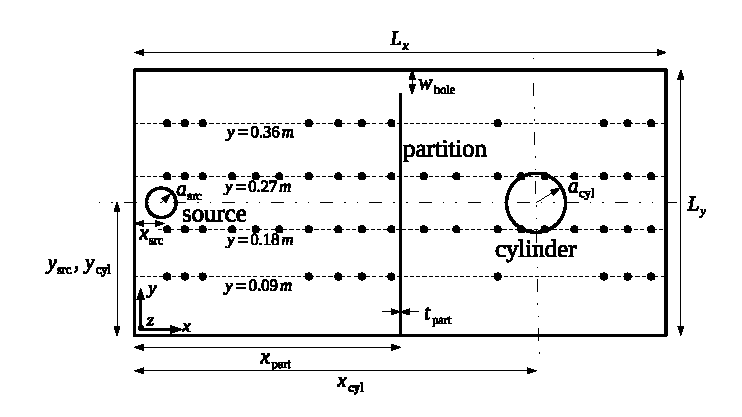
\includegraphics[width=0.8\linewidth]{figures/geometry}
\vspace{-4mm}
\caption{\label{fg:tcgeom} Cross-section in the $xy$-plane of the test case geometry.
The small black dots represent the probe locations in the z=h plane used for the measurements.}
\end{center}
\end{figure}

\begin{table}[ht]
\begin{center}
\begin{tabular}{|c|c|c|}
\hline
\textbf{Parameter}     &\textbf{Variable}      & \textbf{Value} \\
\hline
$L_x$                  &\texttt{Lx}            &0.90\,m \\
$L_y$                  &\texttt{Ly}            &0.45\,m \\
$L_z$                  &\texttt{Lz}            &0.45\,m \\
$x_\mathrm{part}$      &\texttt{partX}         &0.45\,m \\
$t_\mathrm{part}$      &\texttt{partThickness} &0.005\,m \\
$w_\mathrm{hole}$      &\texttt{holeWidth}     &0.04\,m \\
$x_\mathrm{src}$       &\texttt{srcX}          &0.05\,m \\
$y_\mathrm{src}$       &\texttt{srcY}          &0.225\,m \\
$z_\mathrm{src}$       &\texttt{srcZ}          &0.225\,m \\
$a_\mathrm{src}$       &\texttt{srcRadius}     &0.02\,m \\
$x_\mathrm{cyl}$       &\texttt{cylX}          &0.675/{\color{red}0.700\,m} \\
$y_\mathrm{cyl}$       &\texttt{cylY}          &0.225\,m \\
$z_\mathrm{cyl}$       &\texttt{cylZ}          &0.225\,m \\
$a_\mathrm{cyl}$       &\texttt{cylRadius}     &0.05\,m \\
\hline
$P^\rt_\mathrm{src}$   &\texttt{TRP}           &1\,W \\
$\alpha_\mathrm{wall}$ &\texttt{wallAE}        &0.0027 \\
$\alpha_\mathrm{part}$ &\texttt{partAE}        &0.0027 \\
$\alpha_\mathrm{cyl}$  &\texttt{cylAE}         &0.95 \\
\hline
\end{tabular}
\end{center}
\caption{\label{tb:tcparam} Primary parameters and variable names for the test cases.}
\end{table}

\begin{figure}[ht]
\begin{center}
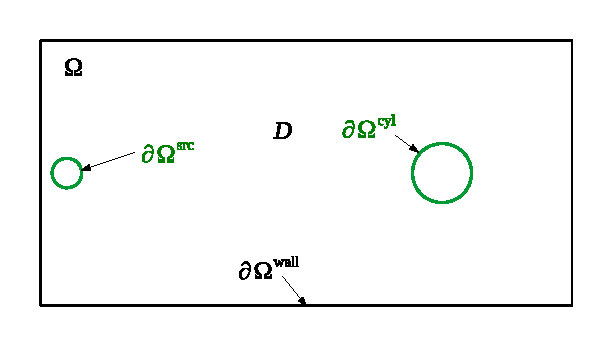
\includegraphics[width=0.6\linewidth]{figures/domains0}
\vspace{-4mm}
\caption{\label{fg:tcdom0} Domain nomenclature for single domain implementation of single cavity.}
\end{center}
\end{figure}

\begin{figure}[ht]
\begin{center}
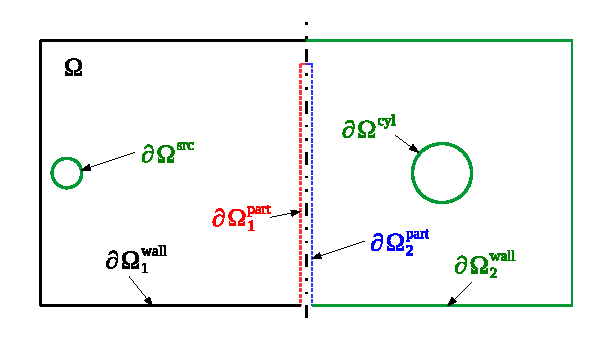
\includegraphics[width=0.6\linewidth]{figures/domains1}
\vspace{-4mm}
\caption{\label{fg:tcdom1} Domain nomenclature for single domain implementation of dual cavity.}
\end{center}
\end{figure}

\begin{figure}[ht]
\begin{center}
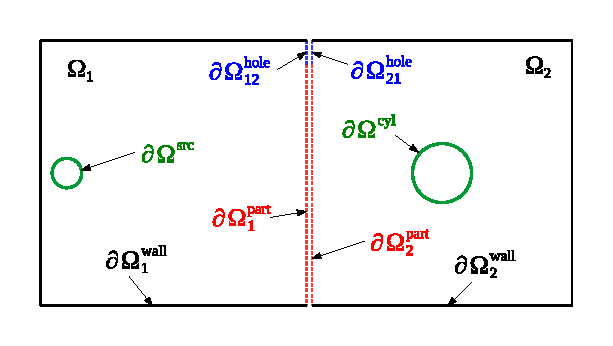
\includegraphics[width=0.6\linewidth]{figures/domains2}
\vspace{-4mm}
\caption{\label{fg:tcdom2} Domain nomenclature for two domain implementation of dual cavity.}
\end{center}
\end{figure}

\bibliographystyle{myabbrvnat}
\bibliography{EDM_Implementation_Notes}

\end{document}
